\subsubsection{Gruppens Sosiale Interaksjon}

Hovedtemaet i denne sekjsonen er å undersøke det sosiale samværet gruppen har hatt, samt diskutere hvilke effekter dette har hatt på gruppen. Her vil gruppen støtte seg til faglitteratur\cite{orgorg}, og se på forhold som særpreger effektive grupper. Busch, Vanebo og Dehlin\cite[p.~257]{orgorg} lister opp en rekkesosiale kvaliteter som er gavnlige for gruppesamarbeid: åpen kommunikasjon, gjensidig tillit, sosial støtte, og utnyttelse av individuelle forskjeller, og disse vil behandles i lys av EiT prosessen. I følgende tekst vil vi prøve og se på det positive og det negative i hver kategori, og prøve og finne ut av hvorfor det sosiale ble som det ble. En gjennomgående faktor i alle kategoriene er gruppens innstilling til EiT fra start av; en positiv, tålmodig og nysgjerrig innstilling til faget har kun hjulpet. Alle disse punktene kan kommenteres på i gruppens sosiale utvikling, og hvilken relasjon dette har hatt til gruppens tilnærming til konfliktbehandling. 

\begin{figure}[h!]
  \caption{Samarbeidsindikator 1, tidlig i faget}
  \centering
    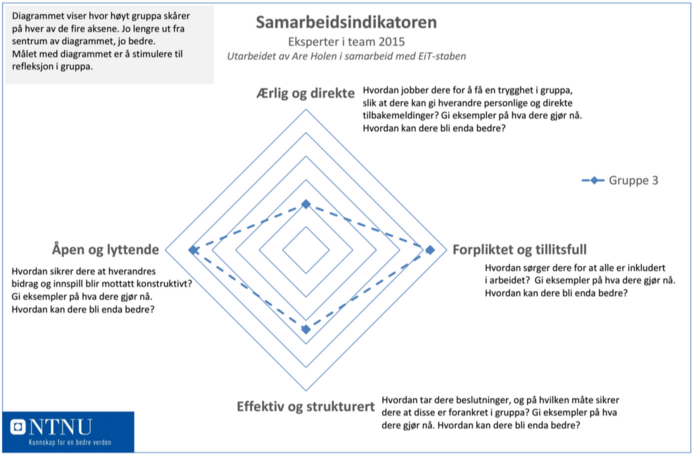
\includegraphics[width=0.5\textwidth]{Bilder/samarbeidsindikator1.png}
\end{figure}\label{samarbeidsindikator1}

\begin{figure}[h!]
  \caption{Samarbeidsindikator 2, midt i faget}
  \centering
    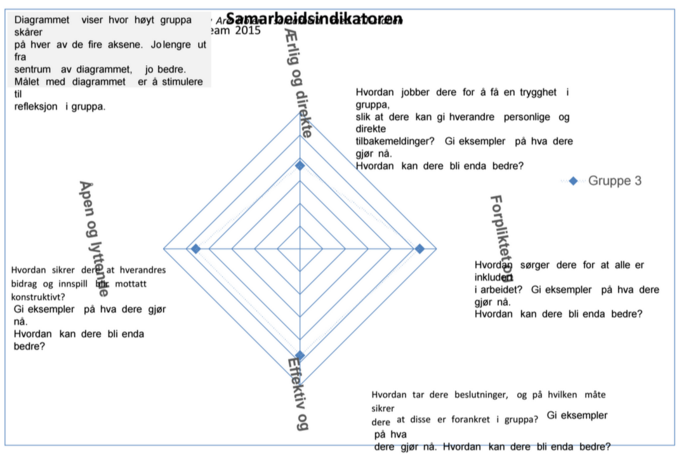
\includegraphics[width=0.5\textwidth]{Bilder/samarbeidsindikator_2.png}
\end{figure}\label{samarbeidsindikator2}

\begin{figure}[h!]
  \caption{Samarbeidsindikator 3, mot slutten av faget}
  \centering
    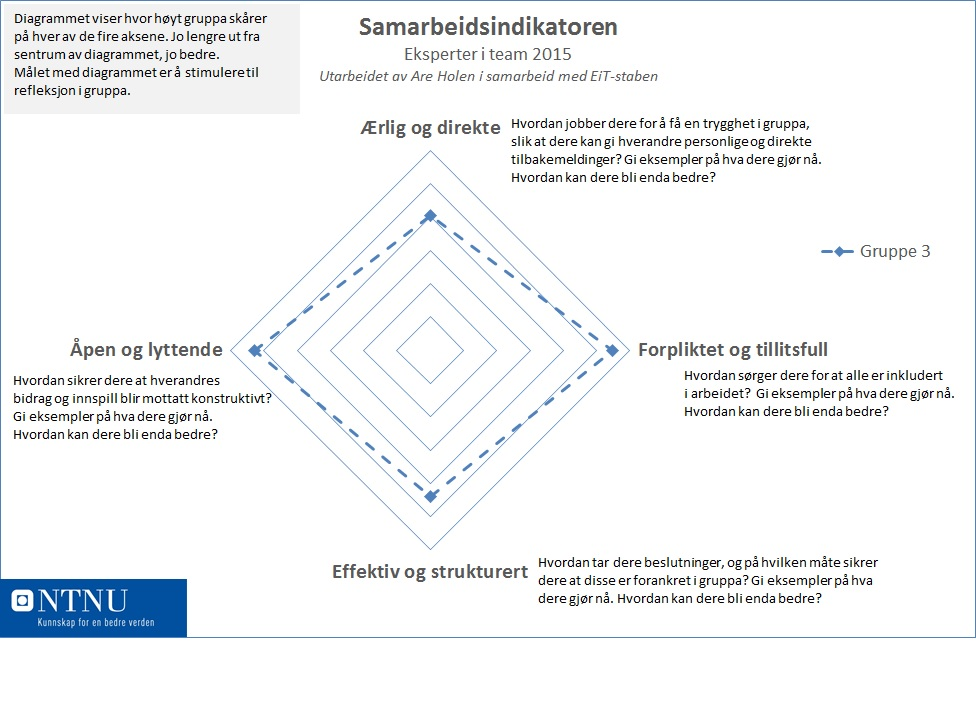
\includegraphics[width=0.5\textwidth]{Bilder/samarbeidsindikator_3.jpg}
\end{figure}\label{samarbeidsindikator3}

\emph{Åpen kommunikasjon} har gruppen hatt bra utslag på ifølge undersøkelsene siden starten av faget\ref{samarbeidsindikator1}. Dette er noe gruppen føler vi har gjort bra, med unntak av oppstartsfasen, og dette må kommenteres på. Her er det dirkekte snakk om gruppens sentimenter omkring ærlig og direkte oppførsel, hvor scoren var lav. Denne dualiteten var noe gruppen stusset over først - vi ble overrasket over den lave ærlighetsscoren, og dette har tydeligvis gjort inntrykk. Scoren for 'åpen og lyttende' atmosfære har vært vedvarende høy, og 'ærlig og direkte' gikk mot mye høyere score\ref{samarbeidsindikator2}, \ref{samarbeidsindikator3}.
Gruppen reflekterte over dette, og kom frem til at det hærsker en spesiell atmosfære når en gruppe er ny, og medlemmene vet at de skal bruke lang tid sammen i arbeidsammenheng. Her vil det ofte være en ivrighet til å skape en god stemning; folk vil le høyere av vitser som de ikke synes er så morsomme, de vil være mere tålmodige med andres bagateller, og være ekstra følsom for å levere en negativ tilbakemelding til noen andre. En analogi kan trekkes til et rom full av diplomater - alle skjønner at ærligheten ofte holdes skjult under en fasade av høflighet, men alle skjønner også at dette gjøres for å sikre en trygg og samtalevennlig atmosfære. Dette forholdet kan justeres på når tilliten mellom diplomatene har vokst. Gruppen mener at en slik stemning var velment, men hindret ærlig og direkte kommunikasjon tidlig i prosessen, og det kom frem i samarbeidsindikatoren.
Dette kunna da også ha bidratt til den trivelige sosiale atmosfæren som kom til; kanskje en startfase hvor ubehageligheter pakkes godt inn i diplomatiske utsagn er noe som skal til for å danne et trygt grunnlag. Som samarbeidsindikatoren viser, så gled gruppen inn i en meget trygg sosial atmosfære, som siden har vært en svært positiv innflytelse på gruppens samarbeid.

\emph{Gjensidig tillit} må opparbeides; det er få situasjoner hvor folk som er hverandre og hverandres bakgrunn fremmed føler seg komfortable før interaksjon. Tillitten i gruppen har kommet av en universell motivasjon for å jobbe sammen - gjennom de mange mindre oppgavene i de første ukene demonstrerte gruppen viljen til både å arbeide og samarbeide. Med en åpen og lyttende natur hvor det har vært ønsket at alle skal bli hørt, har dette ført til en atmosfære av gjensidig tillit. Selv når folk har kommet litt for sent, eller levert ett stykke arbeide for sent, så har det ikke vært foruroligende grunnet den underliggende tilliten. Her kan vi også observere at en øket gjensidig tillit kan føre til at medlemmene er litt mer avslappet rundt tidsfrister. Skulle det være fremmede eller sterkt kritiske kollegaer ville det være mere grunn til sosial stress. Dette ville da kanskje føre til at medlemmene var mere stringent med tanke på frister, men ville skape større sjanse for en potensiellt destruktiv konfrontasjon.

\emph{Sosial støtte} vokste frem stille og rolig, drevet mye av et øket sosialt velbehag, samt innsjekk og utsjekk: de faglig påtvungne innledningene og avrundingene av hver dag som var grobunn for innsikt i hverandres liv utenom det faglige. Derfor ble innsjekk og utsjekk alltid tatt på alvor. I disse 'øyeblikk' har individer fått mulighet til å vise tillit til hverandre og inkludere resten av gruppen i livet sitt. Referatene viser til en trend i å dele 'historier'; gruppen har fulgt Ingelins progresjon i Crossfit, Simens fortellinger om barn og de utfordringer og gleder som følger med, Annas beslutning tidlig i prosessen til røykestopp og maratonløping har utviklet seg som en historie, og Jonas sine ansvar og eventyr på Samfundet er noen eksempler vi kan ta som viser til dette punktet. En god sosial kommunikasjon og en god tone i gruppen hjelper å skape et positiv og trygt arbeidsmiljø\cite{happy}. Medlemmer får lyst å samarbeide og føler seg mer komfortable i samarbeidet, hvis de føler seg verdsatt som mere enn bare et verktøy i et fag.

\emph{Utnyttelse av individuelle forskjeller} på sosialt plan er noe annet en på et faglig plan. Et godt sosialt miljø gjorde at medlemmene ble klar over hvilke personlighetstyper som finnes i gruppen; informasjon som er \emph{svært viktig} i et samarbeid. Fra begynnelsen av prosessen har vært enkelt medlem i gruppen vært inkluderende og dedikerte til laginnsatsen, og dette har gjort det mye lettere å bli kjent med hverandre i lagforbindelse. De forskjellige personlighetstypene ga hver sitt sett med karakteristika som hadde innflytelse, og det blir vanskelig å beskrive bidraget fra de individuelle forskjellene uten å bevege seg i det abstrakte. Her kan man kommentere på Jonas og Karsten sine egenskaper som iværksettere og fremdrivere, hvordan denne har blitt positivt påvirket av Martin og Simens tendens til å være gjennomtenkt og reflektert i sine utsagn, og hvordan alt dette pakkes godt sammen under Anna og Ingelins nøje blikk for struktur og sammenheng. Gruppen hadde også en overordnet tendens til å fremheve den positive siden over den negative siden. Annas usikkerheter rundt det norske språket har ikke vært til bry for gruppen og hun føler seg tålmodig behandlet. På sammen måte \emph{kunne} det vært sett på som en negativ ting at Jonas ofte fører ordet - men gruppen lå heller merke til hvor mye Jonas bidro med. Gruppen har altså ikke latt seg irritere over ting de ikke kunne gjøre noe ved, og heller vært adaptive og kjørt på fordeler og styrker. 